\section{Exact tensor operations and the limits of character constructions}
\label{v7:app:derivations}

This appendix records the finite calculations used in the new sections.
The calculations check identities in representations and in rational
$K$-theory. They do not decide whether a Hodge class on a general fibre
has an algebraic representative.

\subsection{The cube of weights and its two determinant tensors}

The eight weights of the matched fourfold are the vertices of a cube.
The two sets of four vertices in Figure~\ref{v7:fig:cube} are exchanged
by the conjugation of $k$. The columns of the matrix
\[
 W=\begin{pmatrix}
 1&1&-1&-1\\1&-1&1&-1\\1&-1&-1&1
 \end{pmatrix}
\]
are $w_1,w_2,w_3,w_4$. The first three columns have determinant $4$,
and $W(1,1,1,1)^{\mathsf t}=0$. Hence the integral kernel of $W$ is
exactly $\ZZ(1,1,1,1)$. If a zero-weight multiset has multiplicities
$a_i,b_i$ at $w_i,-w_i$, its difference vector is therefore a constant
integer vector. Removing $\min(a_i,b_i)$ opposite pairs at each vertex
leaves whole copies of one tetrahedron. This proves the multiset
assertion for every tensor degree, rather than only the degrees
enumerated by a program.

\begin{figure}[htbp]
\centering
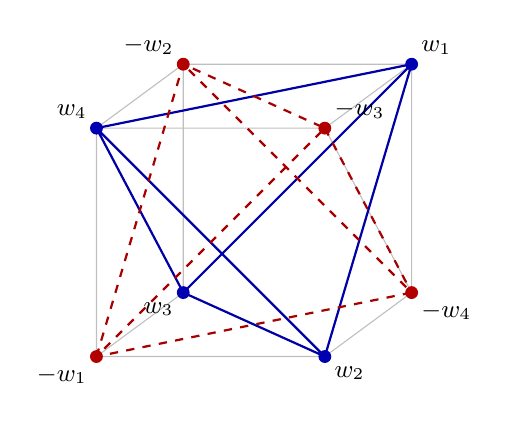
\begin{tikzpicture}[scale=1.45,font=\small]
 \coordinate (a) at (1.38,1.28);
 \coordinate (b) at (.62,-1.28);
 \coordinate (c) at (-.62,-.72);
 \coordinate (d) at (-1.38,.72);
 \coordinate (A) at (-1.38,-1.28);
 \coordinate (B) at (-.62,1.28);
 \coordinate (C) at (.62,.72);
 \coordinate (D) at (1.38,-.72);
 \draw[gray!50] (a)--(B)--(d)--(C)--(a)--(D)--(b)--(A)--(d);
 \draw[gray!50] (A)--(c)--(B) (c)--(b) (C)--(D);
 \draw[blue!65!black,thick] (a)--(b)--(c)--(a)--(d)--(b) (c)--(d);
 \draw[red!65!black,dashed,thick] (A)--(B)--(C)--(A)--(D)--(B) (C)--(D);
 \foreach \p in {a,b,c,d}{\fill[blue!70!black] (\p) circle(1.6pt);}
 \foreach \p in {A,B,C,D}{\fill[red!70!black] (\p) circle(1.6pt);}
 \node[above right] at (a) {$w_1$};
 \node[below right] at (b) {$w_2$};
 \node[below left] at (c) {$w_3$};
 \node[above left] at (d) {$w_4$};
 \node[below left] at (A) {$-w_1$};
 \node[above left] at (B) {$-w_2$};
 \node[above right] at (C) {$-w_3$};
 \node[below right] at (D) {$-w_4$};
\end{tikzpicture}
\caption{A projection of the weight cube. Opposite pairs and the two
tetrahedra generate every zero-weight multiset. The picture describes
the representation at the matched CM fibre; it does not identify
cycles on a generic Mumford fibre.}\label{v7:fig:cube}
\end{figure}

On a power of the fourfold there can be many copies of a weight.
To separate their slots, choose rational endomorphisms on the source
factors and use maps $(x_1,\ldots,x_m)\mapsto\sum f_j(x_j)$.
After scalar extension the endomorphism algebra contains the
individual weight projectors. The pullback of a tetrahedron then
has independently variable coefficients at its four slots.
Coefficient extraction, or a Vandermonde interpolation using rational
parameters, spans every choice of four slots. A polynomial vanishing
on all rational parameters vanishes identically. This explains why
the weight calculation proves generation on all powers, rather than
only on the fourfold itself.

\subsection{Partial symplectic transpose}

In the ordered basis $e\otimes e,e\otimes f,f\otimes e,f\otimes f$
the swap on a two-dimensional factor has matrix
\[
 S=\begin{pmatrix}1&0&0&0\\0&0&1&0\\0&1&0&0\\0&0&0&1\end{pmatrix}.
\]
Write $J=\left(\begin{smallmatrix}0&1\\-1&0\end{smallmatrix}\right)$
for the alternating form. If $t_1$ is ordinary transpose in the first
factor, define
\[
 \tau(A)=(J^{-1}\otimes I)A^{t_1}(J\otimes I).
\]
Direct matrix multiplication gives $\tau(S)=I-S$ and
$\tau((I-S)/2)=S/2$. For a product of operators in the three distinct
colours the transpose factors colour by colour. It is not an algebra
homomorphism on arbitrary endomorphisms, and no such assertion is used.
On the common eigenspace of the three swaps with signs
$\epsilon_i,\epsilon_j,\epsilon_l$, the adjoint projector gives
\[
 \tau(P_i)=\left(1-\frac{\epsilon_i}{2}\right)
            \frac{\epsilon_j\epsilon_l}{4}.
\]
Its square is $1/64$ for $\epsilon_i=1$ and $9/64$ for
$\epsilon_i=-1$, proving the interpolation in
Theorem~\ref{v7:thm:powers}.

For the primitive projector from $\bigwedge^2V$, the corresponding
eigenvalue is
\[
 \frac{\epsilon_i}{2}
  \left(1-\frac{\epsilon_j}{2}\right)
  \left(1-\frac{\epsilon_l}{2}\right).
\]
Its possible values are $\pm1/8,\pm3/8,\pm9/8$.
A polynomial taking value $1$ at the negative values and $0$ at the
positive values recovers $(1-s_i)/2$. The six values are distinct,
so rational Lagrange interpolation supplies this polynomial. Every
coefficient is rational before the scalar extension that separates
the three embeddings of $F$.

\begin{figure}[htbp]
\centering
\begin{tikzpicture}[>=Stealth,node distance=5mm,font=\small,
 b/.style={draw,rounded corners=2pt,text width=33mm,minimum height=12mm,align=center}]
 \node[b,fill=blue!6] (a) {One algebraic\ exceptional class};
 \node[b,right=of a,fill=blue!6] (b) {Cubic action\ and projectors};
 \node[b,right=of b,fill=blue!6] (c) {Partial transpose\ and colour swaps};
 \node[b,below=of b,fill=green!7] (d) {All invariant tensors\ on powers of $X$};
 \draw[->] (a)--(b); \draw[->] (b)--(c);
 \draw[->] (c.south)|-(d.east);
\end{tikzpicture}
\caption{An explicit conditional transfer. The tensor operations are
algebraic; the first exceptional cycle is the missing input at a
full-group fibre.}\label{v7:fig:transfer}
\end{figure}

\subsection{Why a pure mixed character is not an effective sheaf}

Let $Y=X_c^2\times Z_c$, and let $H$ be the sum of ample classes
pulled back from its three factors. Its dimension is fourteen.
The nonzero mixed class $\xi_c$ has K\"unneth degrees $(1,1,2)$,
whereas every term of $H^{12}$ has even degree on each factor.
Integration over $Y$ therefore gives
\begin{equation}\label{v7:eq:zero-degree}
 \int_Y \xi_c H^{12}=0.
\end{equation}

\begin{proposition}\label{v7:prop:no-effective-pure}
The perfect complex in Proposition~\ref{v7:prop:adams} cannot be
replaced by a coherent sheaf with the same cohomological Chern
character. Nor can a vector bundle with character $r+N\xi_c$, with
$r,N>0$, admit a Hermite--Einstein metric for the product polarization
$H$.
\end{proposition}
\begin{proof}
Suppose a coherent sheaf has $\ch_0=\ch_1=0$ and
$\ch_2=N\xi_c\ne0$. Rank zero makes it torsion. Its codimension-one
cycle is effective and represents $\ch_1$. Positivity of degree for
an ample polarization forces that cycle to vanish, so the support
has codimension at least two. Its leading codimension-two cycle is
again effective, with positive lengths at its generic points, and
represents $\ch_2$. If nonzero it has strictly positive intersection
with $H^{12}$, contradicting \eqref{v7:eq:zero-degree}. If it is zero,
then $\ch_2=0$, also a contradiction.

For a rank-$r$ bundle with the indicated character, $c_1=0$ and
$2r c_2-(r-1)c_1^2=-2rN\xi_c$. Its intersection with $H^{12}$ is
zero. In the Chern--Weil equality for a Hermite--Einstein connection
this intersection is a positive constant times the squared norm
of the trace-free curvature \cite{Lub82}. It follows that the
connection is projectively flat. A projectively flat bundle has
$\ch_2=c_1^2/(2r)$, which is zero here, contradicting
$\ch_2=N\xi_c\ne0$.
\end{proof}

Thus clearing denominators and applying Adams operations construct
a perfect complex but do not produce a positive sheaf or a
Hermite--Einstein representative. A construction using stability has
to change the other Chern components as well and check their Hodge
behaviour. This is an obstruction to these particular representatives,
not to algebraicity of the mixed cycle.

\subsection{The character projection and the deformation obstruction}

For $0\le j\le14$, Adams operations act on $\ch_j$ by $2^j$.
The polynomial
\[
 q_2(T)=\prod_{\substack{0\le j\le14\\j\ne2}}
        \frac{T-2^j}{4-2^j}
\]
satisfies $q_2(4)=1$ and $q_2(2^j)=0$ for every other $j$ in this
range. Its coefficients can be checked in $\QQ$ without a cycle
oracle. The construction controls the image in cohomology of a
$K$-class. Deformation of an object representing that class is
governed instead by its Atiyah class and self-extension groups.

\begin{figure}[htbp]
\centering
\begin{tikzpicture}[>=Stealth,node distance=24mm,font=\small,
 b/.style={draw,rounded corners=2pt,text width=40mm,minimum height=13mm,align=center}]
 \node[b,fill=blue!6] (k) {A $K_0$ class\\at the CM fibre};
 \node[b,right=of k,fill=blue!6] (ch) {Pure mixed character\\$N\xi_c$};
 \node[b,below=10mm of k,fill=orange!10] (ext) {$\operatorname{Ext}^2(E,E)$\\Obstruction to deformation};
 \node[b,right=of ext,fill=blue!6] (h) {Cohomological\\obstruction: zero};
 \draw[->] (k)--node[above=8mm]{Adams projection}(ch);
 \draw[->] (k)--(ext); \draw[->] (ch)--(h);
 \draw[->] (ext)--node[below=8mm]{semiregularity}(h);
\end{tikzpicture}
\caption{The bottom arrow can have a nonzero kernel. The explicit K3
example of Theorem~\ref{v7:k3-obstructed-bundle} exhibits a
nonzero obstruction in that kernel despite preservation of the
entire Chern character.}\label{v7:fig:obstruction}
\end{figure}

The file \path{checks/check_weights.py} verifies the subset counts
for $\bigwedge^3V$ and $\bigwedge^4V$, the matched CM weight
multiset, the two-dimensional partial-transpose matrix identities,
all fifteen Adams eigenvalues, and the ranks of the root
intertwining systems. All arithmetic in that file is exact.
The infinite-degree multiset argument, the existence of the CM
embedding, the algebraic projector construction and the deformation
arguments are proved in the text. The finite checks neither
formalise those geometric proofs nor establish \Fii{} or \Fiii{}.
